\setchapterpreamble[u]{\margintoc}
\chapter{Renewables}
\labch{renewables}

A renewable energy is an energy source that is replenished at least as fast as it can be used. In other words, it depends on the timescale involved, and that timescale needs to be on the human, rather than geological scale. As you know, solar and wind are considered fully renewable. As long as the sun exists, and as long as Earth has an atmosphere, we will have solar radiation and wind mechanical force to potentially harvest. Water is another such resource, with evaporation and condensation (water cycle) taking care of the replenishment of our fresh water reservoirs. Biomass, also known as vegetation, is renewable, up to what can be regrown on the order of the yearly scale.

So, an interesting thing to note is that solar energy is the basis of every single renewable energy source on Earth. The wind exists because of a temperature gradient, caused by the sun irradiance. The water cycle exists because of the evaporation and rainfalls, caused by the warmth brought by the solar rays. The biomass develops by capturing the sun energy by photosynthesis. Only one renewable energy does not depend on the sun, and that is geothermal energy, but the challenges of tapping into that resource are immense. Note that (we will expand on this) current geothermal installation tap into the limited surface flux, not the actual heat reservoir.

Fossil energies are also replenished over time, but on a timescale that are disqualifying for renewable resources. Nuclear energy is also not a renewable energy due to the finite amount of uranium or thorium notably. However, those resources are vast, which leads some to consider it as a honorary renewable energy due to its capacity at generating a lot of power with little carbon emissions. This is however not technically accurate. Some also equate nuclear fuel with fossil fuels due to the fuel mining necessary. This is also false.

Renewable energies are not all equal, both in terms of their capture or their efficiency, as well as localized variability. As a quick illustration, hydroelectric power is a renewable energy because of the water cycle replenishing the reservoir. However, at the same time, its capture and transformation to electricity is limited in terms of scale due to a limited number of siting locations available in the world. The resource itself (water) is thus renewable, but the means of capture is not.

Understandably, renewable energies have been touted as the savior for humanity for as long as we have known that fossil fuels were a problem, which is, as we have noted previously, much longer than people tend to realize. The main reason for this is two-fold. They seem to be getting back to a natural order of things, a less industrialized period, and the theoretical potential is incredible and dwarf (for solar notably) any other energy source. In a little under two hours, enough solar energy strikes the Earth to power our world society for a year.

\begin{figure}[h]
	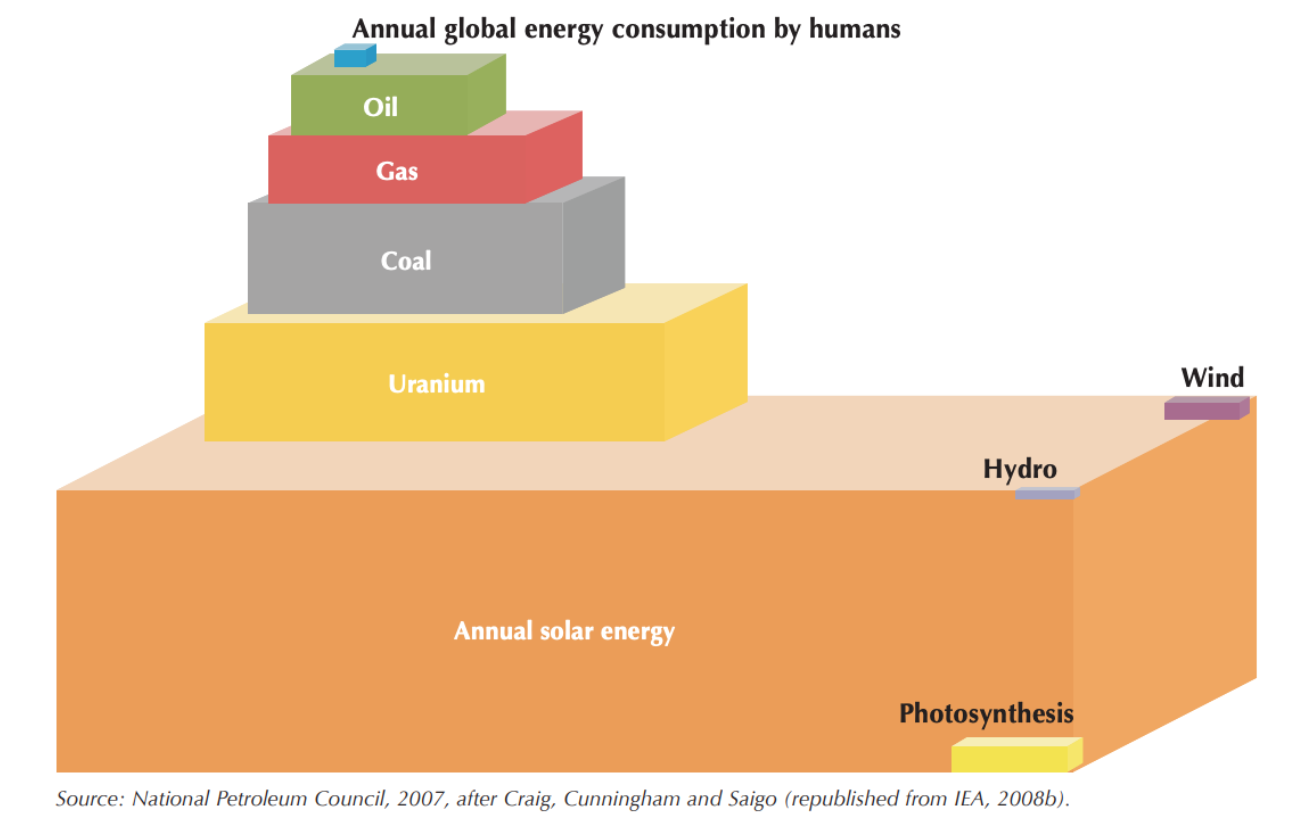
\includegraphics[width=1.0\textwidth]{power_generation_potential_sources}
	\caption[Representation of the potential energy from different sources]{Representation of the potential energy from different sources.}
	\labfig{power_generation_potential_sources}
\end{figure}

It is consequently tempting to think that it is a simple matter of capturing it. But that capture is everything but simple.

Today, if you were to think about it quickly, or ask almost anyone in the streets, the question “What is renewable energy?”, the first two responses by far would likely be “solar” and “wind”. In reality, those two account for a very small fraction of the renewable energy mix, which is dominated by hydroelectricity and by the biomass. Right now, you should not really picture a solar panel or a wind turbine, but a dam or a forest, especially historically.

\section{Biomass}

Biomass energy is limited by the deforestation rate. In other words, in order for the biomass energy to be considered renewable, one must not deplete the forests at a higher rate than photosynthesis replenish them.

\section{Solar}

Direct heating from sun irradiance through windows is a big natural use. Having houses that are able to do that is important, but retrofitting is not really an option. Solar heating of air or water can also be a use of solar energy, notably for showers or house flooring. Finally, the electrical conversion through photovoltaic panels can be done.


\section{Wind}

\blindtext

\section{Hydroelectricity}

Hydroelectricity is the largest renewable source of electricity in use today. It represents a very large share of electricity production in several countries, lucky enough to have the necessary terrain.

The principle of hydroelectricity is simple. It is all potential energy. The power is relative to the gravitational force, which is unfortunately not very dense.

\begin{kaobox}

If $m$ is the mass of water in the reservoir, $g$ the gravitational acceleration constant and $h$ the height of the reservoir, then the potential energy stored in our reservoir is given by~\ref{potential_energy}\footnote{Mind the units!}.

\begin{equation}\label{potential_energy}
E = m \times g \times h
\end{equation}



\begin{itemize}
\item A single AA battery is roughly equivalent to lifting 100 kilogram of water up 10 meters
\item A gallon of gasoline is roughly equivalent to lifting 1.3 tons of water up 10 meters
\item A gram of Uranium-235 is roughly equivalent to lifting 1.3 tons of water up 8 kilometers\sidenote[][-2mm]{Another way to look at it is taking 2 CESSNA-172 (around 1.3 tons each) up to cruising altitude (around 4km)}
\end{itemize}

\end{kaobox}

So, with hydroelectricity, we are simply talking of getting water at an altitude and make it go down through turbines, hence delivering their potential energy. In order for this to work at scale, we have to consider very large volumes. Volume is only one part of the equation though, height is another one. This is the reason why you usually find large hydroelectric facilities in mountainous terrain. Run-of-rivers facilities are another option, this time taking advantage of the natural reservoir created by the flowing river.

The water is replenished in the reservoirs (lakes, rivers) by the water cycle. Consequently, this resource, while fully renewable, is limited in its capture by the rate of condensation in the basin. Drought notably impacts water height and consequently the power capacity of a dam.

\section{Geothermal}

\blindtext


\blindtext


\section{The Digest}


\begin{kaoboxgreen}[frametitle=Main Takeaways]

\begin{itemize}
\item Biomass is rate-limited and can have alternative carbon uses. It is also important as a human-nature barrier.
\item Solar is fun, and can be useful, but stay reasonable with the hype, and its non controllability is an issue
\item Wind is a really nice technology, but its non controllability is an issue
\item Hydroelectricity is the main renewable energy in use today, and would be fantastic if it were not for pesky physics
\end{itemize}
  
\end{kaoboxgreen}